\section{Bond Lengths}

A simple analysis of atomic distances within the malonic acid molecule verifies the expected equilibrium lengths and geometry. Looking at the acid alcohol moiety's O-H distance also verifies the protonation state to ensure that the imposed low-pH conditions effectively keep the surface malonic acid fully protonated throughout the simulations. The bondlength trajectory of the acid O-H bond is plotted in Figure \ref{fig:bondlength-trajectory} (dark blue and green traces) for both of the carboxylic acid moieties of two representative simulations. Both O-H distance traces remain very close to the expected equilibrium O-H covalent bondlength of 1\angs for the entire trajectory, indicative of a protonated acid. All five simulated malonic acids were verified to be fully protonated throughout the trajectories.

\begin{figure}[h!]
	\begin{center}
		\includegraphics[scale=1.0]{images/bond-length/bondlengths.png}
		\caption{}
		\label{fig:bondlength-trajectory}
	\end{center}
\end{figure}

Each permutation of atomic pair distance trajectories was inspected, and a noteworthy atomic bonding pattern occured in two of the five simulations. Figure \ref{fig:bondlength-trajectory} also shows the plots of distances between each acid proton and the carbonyl oxygen on the opposite end of the molecule (in red and light blue). The top plot of Figure \ref{fig:bondlength-trajectory} shows the case where one of the two \ocarb~distances is significantly shorter than the other, spending nearly the entire trajectory with a bond distance of a strong hydrogen bond. The bottom plot shows a simulation where both \ocarb~distances remain longer than an H-bond. The former case (top plot) is hereafter referred to as the ``internally bonded'' or ``intramolecularly H-bonded'' molecule, and the latter case (bottom plot of Figure \ref{fig:bondlength-trajectory}) is referred to as the ``internally unbonded'' malonic acid. A graphic depiction of the proposed structure of these two geometries is shown in Figure \ref{fig:bondlength-trajectory}, with the internally bonded form exhibiting an intramolecular hydrogen bond interactio between one acid hydrogen and a carbonyl oxygen at the opposite end of the molecule. The bondlength plots of Figure \ref{fig:bondlength-trajectory} show color-coded circles around each bond of the molecular graphic to the right of the plots to designate each trace.

Referring to Figure \ref{fig:bondlength-trajectory}, the presence of a hydrogen bond internal to the acid folds the molecule into a ring-like structure of six atoms. The intramolecular H-bond is strong enough to persist for the entire length of two of the five simulations, and forms at some time during the equilibration phase of simulation. Conversely, in the simulations exhibiting internally unbonded molecules, the intramolecular H-bond forms only briefly, or not at all during the entire simulated trajectories. Additionally, all simulation cells were initialized with malonic acids with identical internal geometries, albeit randomly placed and oriented on the water surface. This suggests that the formation of the internally bonded configuration is a result of the initialplacement of the acid with respect to the simulated water molecules in the system, i.e. the initial solvation of the acid.

The unique internal behavior of malonic acid is thus established with two of the five simulations exhibiting the internally bonded configuration. The other three simulated acids remained internally unbonded. For the remainder of this work we present results for both sets of simulations, as well as the collection of all simulations, to highlight similarities and differences between them, in order to show trends in the behavior of malonic acid on a water surface.

Figure \ref{fig:bondlength-distribution} shows the distribution of bondlengths for the covalent O-H bonds, the \ocarb~distances, and also the C=O carbonyl bonds, using the same color scheme as in Figure \ref{fig:bondlength-trajectory}. The top plot shows the bondlength distribution for the internally H-bonded malonic acid simulations, and the bottom plot shows the distributions for the internally unbonded acid molecules. The insets of Figure \ref{fig:bondlength-distribution} expand on the region containing the O-H alcohol, and C=O carbonyl moieties. The bondlength distribution plots further emphasize trends noted earlier, and show other configurational changes in the malonic acid molecules.

\begin{figure}[h!]
	\begin{center}
		\includegraphics[scale=1.0]{images/bond-length/BondLengthDistros.png}
		\caption{}
		\label{fig:bondlength-distribution}
	\end{center}
\end{figure}

The bottom plot of Figure \ref{fig:bondlength-distribution} shows each of the three types of bonds (O-H, \ocarb, C=O). Each pair of distributions corresponding to each bond type are of similar width and overlap because they each have very similar peak locations. This is indicative of a malonic acid where both ends of the molecule behave similarly, most likely due to similar hydration environments. This also suggests that the internally unbonded malonic acid orients symmetrically with respect to the water surface in order to achieve equal solvation for both carboxylic acid groups (i.e. the acid lies flat in the plane of the surface keeping both carboxylic acids at equal depths). 

The case of the internally bonded acid molecule (bottom plot of Figure \ref{figbondlength-distribution}) is different in many respects. Firstly, the distribution of the bondlengths at both ends of the molecule are distinct such that one peak of each bond type distribution is centered at a longer bondlength than the other (e.g. one of the C=O carbonyl bondlengths distributions is shifted to the right relative to the distribution of the other carbonyl in the opposite carboxylic acid group). With regards to the internal hydrogen bond, the light blue peak is entirely below a typical H-bond length in water (approximately 2.4\angs), whereas the other \ocarb~distance is greater than 4\angs. Interestingly, there are two distinct peaks in the non-bonding \ocarb~distribution (red trace) indicating two distinct conformations of the internally bonded malonic acid. These conformations bring the unbound \ocarb~closer or further away at different times during the simulations.

The presence of the intramolecular H-bond affects the covalent bonding throughout the malonic acid. Looking at the two O-H peaks centered near 1\angs, one is shifted to longer bondlengths (green) than the other (dark blue). The green colored trace of Figure \ref{fig:bondlength-distribution} corresponds to the alcohol moiety that is participating in the internal hydrogen bond. The delocalization of the bonding electrons in a hydrogen bond allows the hydrogen proton to move further from its covalently bound oxygen, shifting the bondlength distribution to the right relative to the unbonded O-H (colored dark blue). Consequently, the C=O carbonyl bonds behave similarly. The maroon colored bondlength distribution corresponds to the H-bonded carbonyl oxygen. The entire bondlength distribution is shifted to the right of the carbonyl not participating in the internal H-bond (yellow trace). The peak centers and widths of the distributions are listed in Table \ref{table:peaks}, quantifying the changes to the bondlengths. These geometric changes result in other behavioral differences, both orientationally and spectrally, as described later in this work.
